%--------------------------------
%RESULTADOS
\section{Region Segmentation Experiments}
\label{cap6_result_experm_1}

The first set of experiments aimed to analyze the feasibility of the method described in Section \ref{cap5_metodologia}.
For an initial analysis, the region segmentation task was considered more appropriate, as it requires a lower level of precision than edge detection problems.
Also, it was evaluated the influence of the amount of side-outputs and the performance of the methods to combine them.

The experiments were conducted using the KITTI Road/Lane data set.
This data set is composed of 289 training and 290 test images with size of $1242 \times 375$ pixels. 
Ground truth is manually annotated for two different pixel types: $(i)$ \textbf{road} is the area of the road that makes up all lanes; and $(ii)$ \textbf{lane} is the ego-lane where the vehicle is currently in \cite{Fritsch2013ITSC}.

KITTI data set contains only ground truth for training data.
The test set is evaluated using the KITTI Server Evaluation.
In the work developed, only road markings were considered and images for lane segmentation were ignored.
The ground truth of roads is divided into three categories: $(i)$ urban unmarked (\textbf{uu\_road}), $(ii)$ urban marked (\textbf{um\_road}), $(iii)$ urban multiple marked lanes (\textbf{umm\_road}) \cite{Fritsch2013ITSC}.

To increase the number of images in the training set, data-augmentation techniques were used.
The following transformations have been applied: salt/pepper noise, noise shadow, horizontal inversion (mirroring), contrast and brightness change, random rain/snow addition.
Data augmentation procedures that create unwanted behavior, such as vertical inversion and distortions that would change the nature of objects in the scene, such as cars and pedestrians, have been avoided.
Enlargement procedures resulted in 2601 images, divided into 2080 training samples and 521 validation samples (about 20\%).

The initialization of weights was based on a pre-trained VGG16 model\footnote{VGG16 model was trained using ImageNet dataset \cite{ILSVRC15}.}.
In addition, we use Stochastic Gradient Descen (SGD) optimization with $1 \times 10^{-3}$ learning rate, $5 \times 10^{-6}$ learning decay and 0.95 momentum.
To tune the network and speed up the process, all images have been scaled down to $624 \times 192$ pixels (about 50\%). 
The default batch size had 16 images.

%--------------------------------
\subsection{Influence of merging methods and the number of side-outputs}
\label{cap6_experm_1_qtd_saidas}

The first test of the current experiment was designed to identify the influence of the number of side-outputs and the best merging methods.
For this, it were used \textbf{ALO} and \textbf{SLO} networks, detailed in Section \ref{cap5_saidas_laterais}.
The networks have been trained for only 100 epochs, using each merging methods.
It was also used a modified VGG16 version to predict regions, without side-outputs, as baseline, called in this work \textit{No Side-Outputs} (\textbf{NSO}).
%Figure \ref{fig:kitti_validation_loss_100epochs} shows the loss curves during the training phase for the validation set.

% \begin{figure}
%   \centering
%   \caption{Validation loss using \textit{Categorical Cross Entropy} metric.}
%   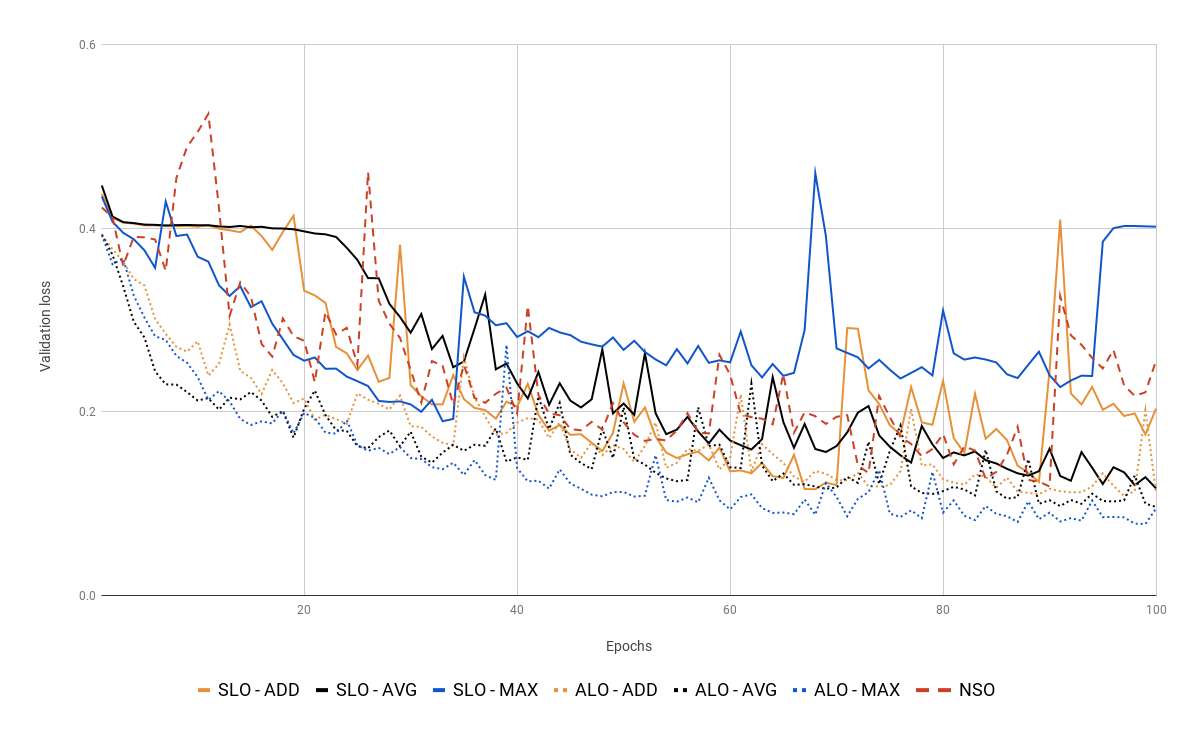
\includegraphics[width=1.\columnwidth]{../../imagens/graficos/cap6_kitti_validation_loss.png}
%   \sourceOwn
%   \label{fig:kitti_validation_loss_100epochs}
% \end{figure}

It is observed in the first part of the experiment that the ALO networks appear to be more stable, with a steeper loss curve than the NSO and all SLO approaches.
% In addition, it is important to note that the NSO and SLO-MAX networks are highly unstable during learning phase, with abrupt changes in the loss value, resulting in graphical spikes.
In addition, NSO and SLO-MAX networks were highly unstable during learning phase, with abrupt changes in the loss value, resulting in graphical spikes.
On the other hand, the ALO-AVG network had the best result, followed by ALO-MAX and ALO-ADD.
This is possibly caused by the considerably higher number of outputs, which creates the possibility of exchange between confident values.

To improve results, a new round of testing was created with 500 training epochs.
As SLO networks showed poor performance in the previous test and other tests performed with different parameters, then it was decided to evaluate only ALO networks.
The network NSO was also trained as a comparison \textit{baseline}.

Performance analysis was done by two different metrics: the well-known \textit{Categorical Cross Entropy} and \textit{Pixel-error} metric.
Pixel-error was adopted when high precision values were observed in results where there were noticeably many errors, especially with numerous false positives.
% The performance of the above networks using both metrics is shown in Figures \ref{fig:kitti_cross_entropy_500_epochs} and \ref{fig:kitti_pixel_error_500_epochs}. 
%It can be observed that side-outputs have a positive influence on the performance of the networks.
All versions of network ALO outperforms NSO network using both metrics.

% \begin{figure}
%   \centering
%   \caption{Performance of ALO and NSO nets using \textit{Categorical Cross Entropy} metric.}
%   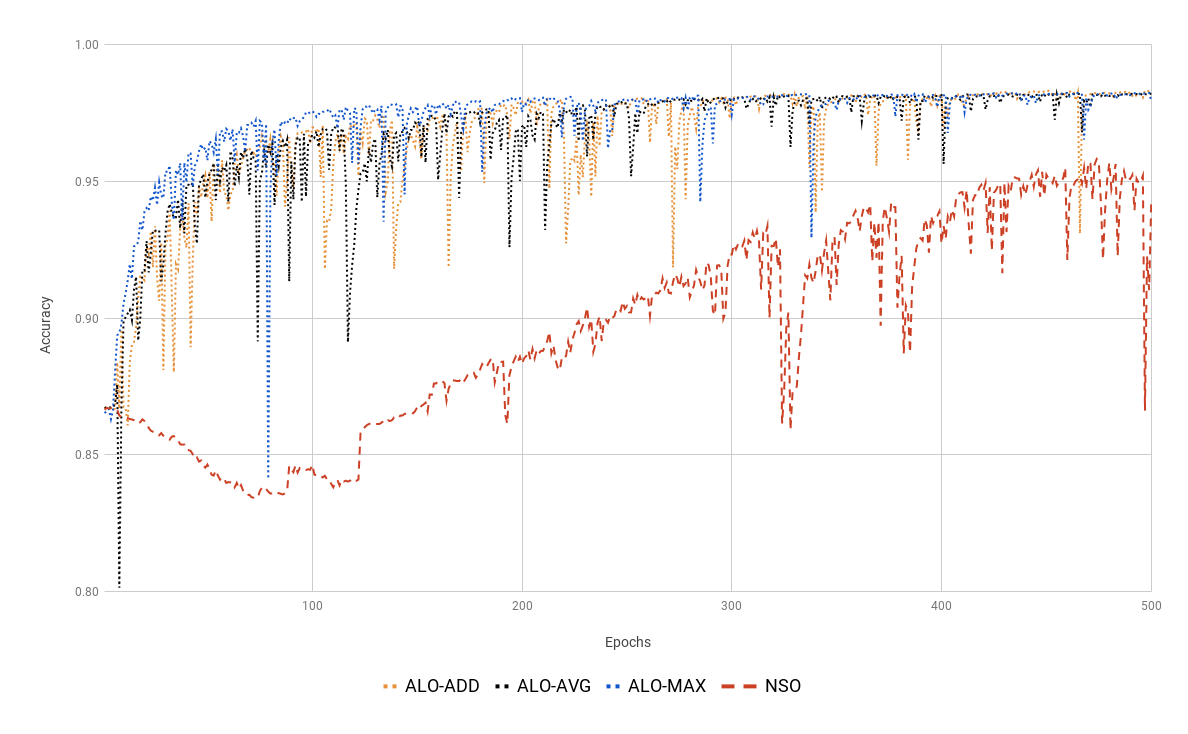
\includegraphics[width=1.\columnwidth]{../../imagens/graficos/cap6_kitti_val_acc_500_epochs.png}
%   \sourceOwn
%   \label{fig:kitti_cross_entropy_500_epochs}
% \end{figure}
% 
% \begin{figure}
%   \centering
%   \caption{Performance of ALO and NSO nets using \textit{Pixel-Error} metric.}
%   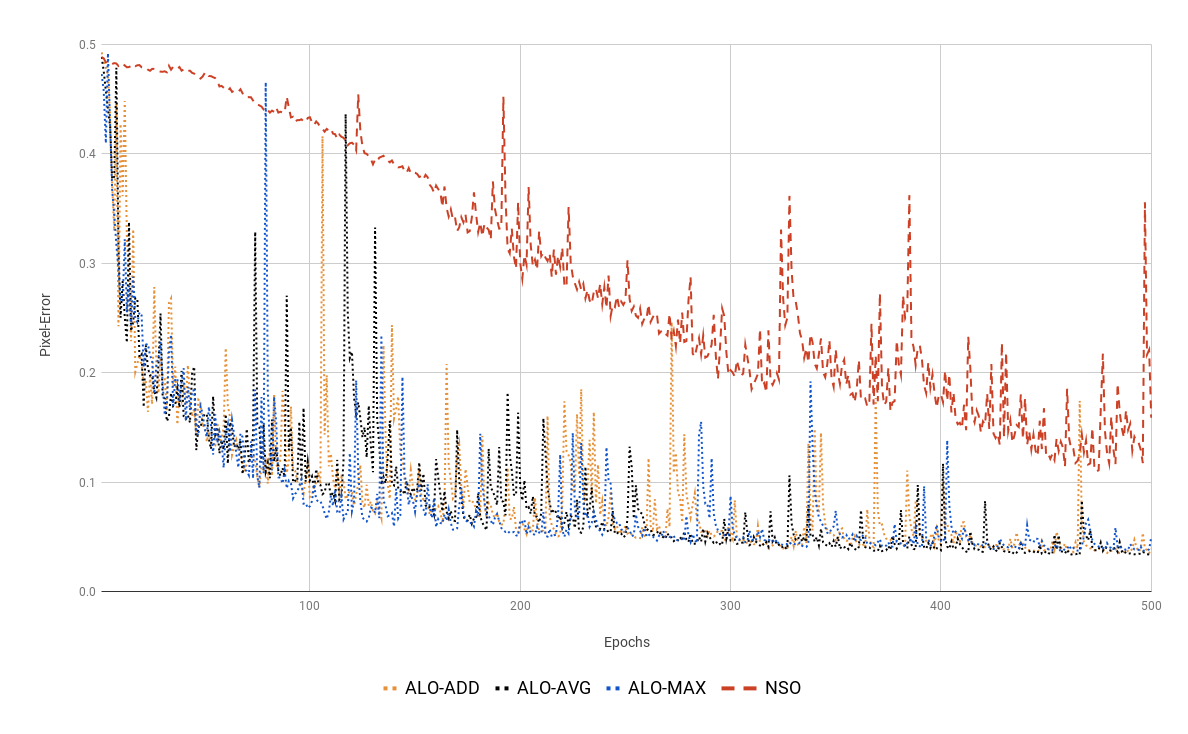
\includegraphics[width=1.\columnwidth]{../../imagens/graficos/cap6_kitti_pixel_error_500_epochs.png}
%   \sourceOwn
%   \label{fig:kitti_pixel_error_500_epochs}
% \end{figure}

The results of the merging techniques of the ALO networks have similar value, indicating the absence of a considerably superior method to the others.
The best result for \textit{Categorical Cross Entropy} metric slightly outperforms the worst method (0.983 for ALO-ADD and 0.9821 for ALO-AVG).
Using \textit{Pixel-error metric}, the best value is only 0.004 higher than the worst (0.0332 for ALO-AVG and 0.0372 for ALO-MAX).

%--------------------------------
%SUB - CONTRIBUIÇÕES SAÍDAS laterais
\subsection{Side-Outputs Contribution}
\label{cap6_contribuicoes_saidas_intermediarias}

The layers in each merging strategy learn uniquely.
The contributions to the final prediction differ according to the merging method adopted, as shown in Figure \ref{fig:kitti_side_outputs}.
To make the analysis of the image clearer, only last side-output maps of each stage were plotted.
In addition, the images were transformed into monochromatic (binary), with white pixels representing the road and black pixels representing the background.

% \begin{figure*}
%   \centering
%   \caption{Side-output maps for ALO network merging strategies in KITTI Road/Lane data set.}
%   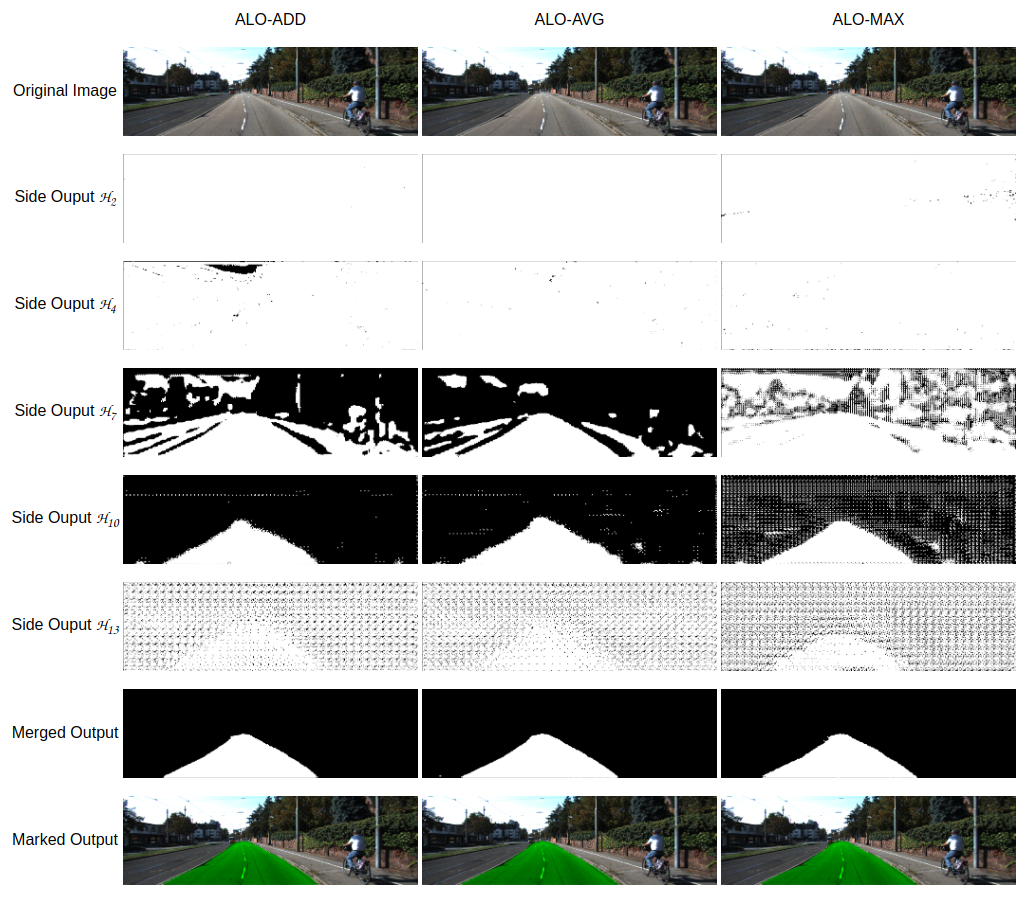
\includegraphics[width=0.7\textwidth]{../../imagens/ilustracoes/cap6_kitti_side_outputs.png}
%   \sourceOwn
%   \label{fig:kitti_side_outputs}
% \end{figure*}

\begin{figure}
  \centering
  \caption{Side-output maps for ALO network merging strategies in KITTI Road/Lane data set.}
  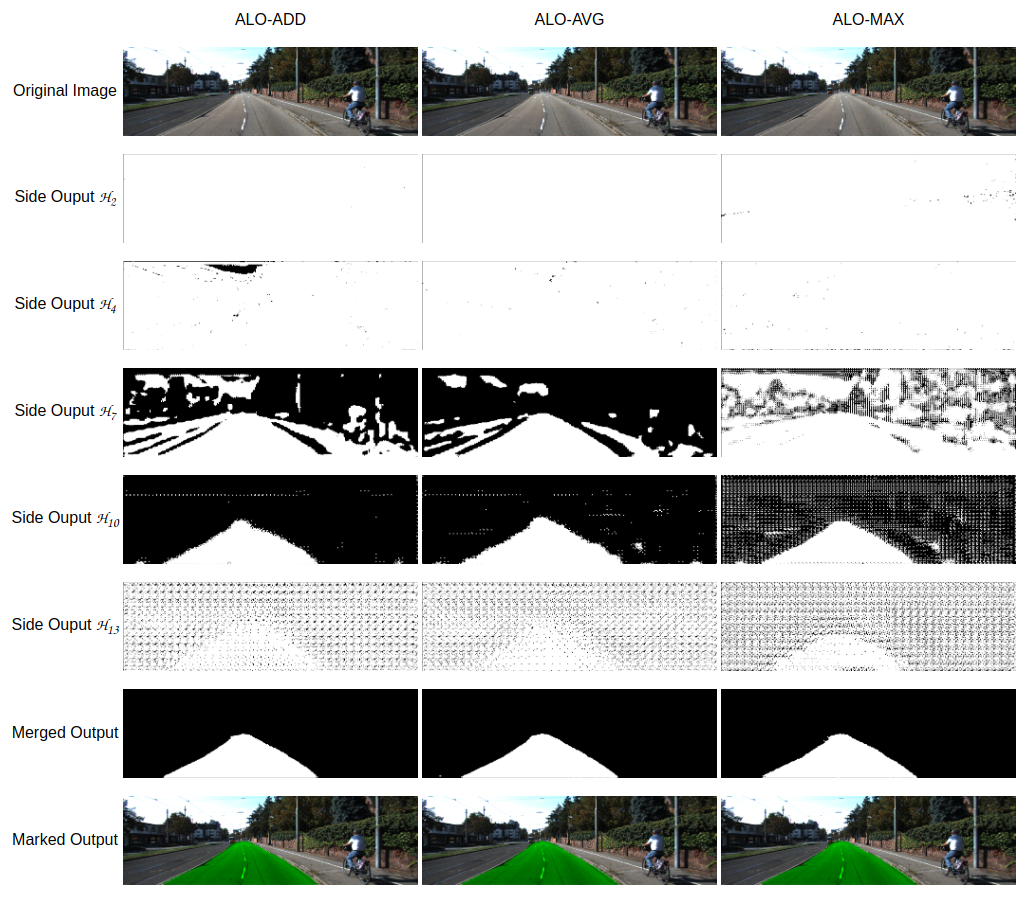
\includegraphics[width=1\columnwidth]{../../imagens/ilustracoes/cap6_kitti_side_outputs.png}
  \sourceOwn
  \label{fig:kitti_side_outputs}
\end{figure}

It can be seen from Figure \ref{fig:kitti_side_outputs} that the first two stages ($\mathcal{H}_2$ and $\mathcal{H}_4$) side-outputs does not produce meaningful information.
The images have mostly white pixels, indicating classification of all pixels as road.
In the third stage (output $\mathcal{H}_7$), the merging methods ALO-AVG and ALO-ADD, contains a obvious separation between road pixels and the background.
The output map $\mathcal{H}_7$, using ALO-MAX method, however, does not clearly separate road from non-road pixels.

Figure \ref{fig:kitti_side_outputs} further shows that the best side-output maps for all networks ALO are generated in the fourth stage $\mathcal{H}_{10}$. 
Road markings are visible even if there are noises, especially in the ALO-MAX method.
The final side-output, $\mathcal{H}_{13}$, contains high noise level.
This feature indicates that the layer was not able to learn correctly.

The merged output combines all side-outputs, including other intermediate results not available in Figure \ref{fig:kitti_side_outputs}, for prediction.
Despite the poor results in some layers, the learning process adjusts itself so that even bad results can be used by the model.

%--------------------------------
%PÓS PROCESSAMENTO
\subsection{Post Processing}
\label{cap6_pos_processamento}

At the end of the segmentation, a post processing step was added to reduce some noise.
For this, the \textit{morphological opening} operation was used to remove small noises created by the foreground (road) in the background.
The operation was applied using a $13 \times 13$ square structuring element as a result of empirical tests.

% A simple comparison of the final result with the original prediction is presented in Figure \ref{fig:kitti_post_processing_comp}.
% The image shows an example of benefit from the post processing step.
% It's possible to see the noise removal mainly at the right edge of the image (\textit{white pixels}).
% A side effect is the removal of some points that seem to fit properly, mostly in lower left and lower right corners of the road (\textit{red pixels}).
% 
% \begin{figure}%[h!]
%   \centering
%   \caption{Differences between original method results and after post processing.}
%   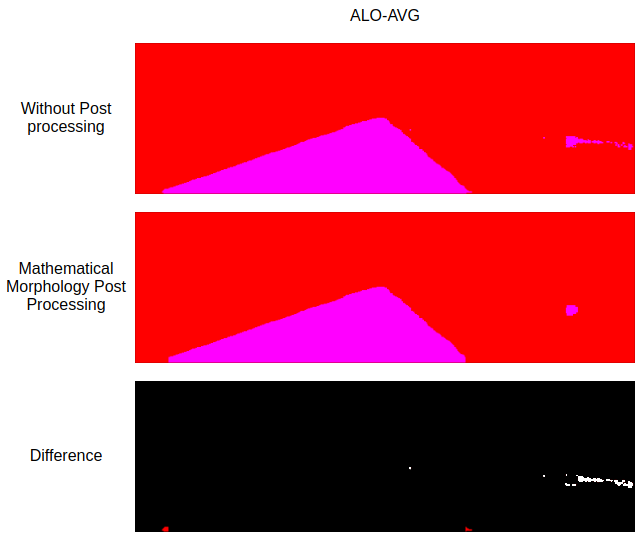
\includegraphics[width=0.9\columnwidth]{../../imagens/ilustracoes/cap6_kitti_post_proc_comp.png}
%   \sourceOwn
%   \label{fig:kitti_post_processing_comp}
% \end{figure}

%--------------------------------
%SUB - RESULTADOS DA SEGMENTAÇÃO
\subsection{Segmentation Evaluation}
\label{cap6_resultados_segmentacao}

After the post-processing step, segmentation quality was evaluated.
The tests were performed using the ALO-AVG method, the best in the training phase.
Results were sent to  the KITTI Evaluation Server, with name of \textbf{ALO-AVG-MM}\footnote{~Results are available in a public leaderboard at \url{http://www.cvlibs.net/datasets/kitti/eval_road.php}}.
The server returned the following metrics: MaxF, AP, PRE, REC, FPR and FNR, whose results for each road scene category\footnote{~\textit{URBAN\_ROAD} category corresponds to the combination of the other three categories.}, as described in Section \ref{cap6_result_experm_1}, are available in Table \ref{tab:kitti_metrics}.

%table kitti_metrics
\begin{table}
  \centering
  \scriptsize
  \setlength{\tabcolsep}{0.8em}
  \renewcommand{\arraystretch}{1.7}
  \begin{tabular}{{l}{c}{c}{c}{c}{c}{c}}
    \hline
    \textit{Benchmark} & MaxF & AP & PRE & REC & FPR & FNR
    \\
    \hline
    UM\_ROAD & 91.15\% & 83.82\% & 89.07\% & 93.33\% & 5.22\% & 6.67\%
    \\
    UMM\_ROAD & 94.05\% & 90.96\% & 94.82\% & 93.29\% & 5.60\% & 6.71\%
    \\
    UU\_ROAD & 89.45\% & 79.87\% & 85.40\% & 93.90\% & 5.23\% & 6.10\%
    \\
    \hline
    URBAN\_ROAD & 92.03\% & 85.64\% & 90.65\% & 93.45\% & 5.31\% & 6.55\%
    \\
    \hline
  \end{tabular}
  \caption{Segmentation performance on KITTI Road Dataset.}
  \label{tab:kitti_metrics}
\end{table}


%The results available in Table \ref{tab:kitti_metrics} show how efficient the method is.
Compared to the best result on the KITTI platform named PLARD \cite{Chen:2019}\footnote{~At the time of our first conference paper submission, \cite{Reis:2019}, \textit{PLARD} had not yet been published in the literature, being an anonymous submission on KITTI platform.}, our method had an overall performance 5.0\% lower.
It is also necessary to remember that the model was trained for only 500 epochs.
Thus, it is indicated that the techniques for combining side-outputs had good results, as desired.

To show the performance of our model, Figure \ref{fig:kitti_representacao_visual} was created with ALO-AVG-MM predictions\footnote{~More visual results are public available on \href{http://www.cvlibs.net/datasets/kitti/eval_road_detail.php?result=a5ca173550cb383caf3e12ca236d7c809489d2d9}{KITTI Server}.}.
Pixels have been labeled as true positives (\textit{green}), false negatives (\textit{red}) and false positives (\textit{blue}).
The original images were created by the KITTI Evaluation Server, based on the binary map sent to the server.

%\begin{sidewaysfigure}
\begin{figure}
  \centering
  \caption{Visual representation of ALO-AVG-MM predictions}
  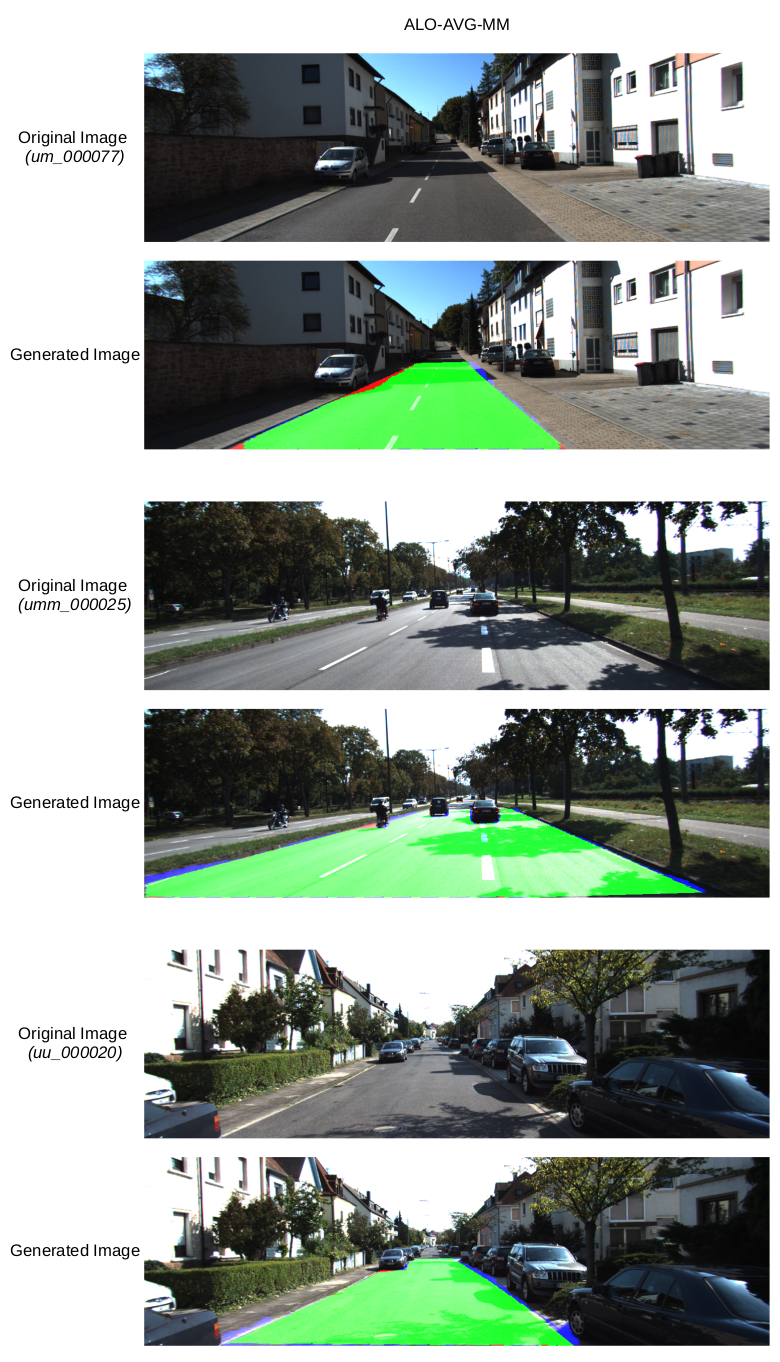
\includegraphics[width=0.9\columnwidth]{../../imagens/ilustracoes/cap6_kitti_visual_representation.png}
  \sourceOwn
  \label{fig:kitti_representacao_visual}
\end{figure}
%\end{sidewaysfigure}
%--------------------------------
